\documentclass[man]{apa2}

\usepackage{pdfsync}
\usepackage{apacite}
\usepackage{amsmath}
\usepackage{graphicx}
\usepackage{topcapt}
\usepackage{color}
\usepackage{inputenc} 
\usepackage{float}


\title{The role of social information in cross-situational word-learning

(Submitted for the First-Year Project)}
\author{Kyle MacDonald}
\affiliation{Department of Psychology, Stanford University}

\vspace{3.0ex}

\shorttitle{Social cues and cross-situational word-learning}
\rightheader{SOCIAL INFORMATION AND CROSS-SITUATIONAL LEARNING}
\leftheader{Kyle MacDonald}

\begin{document}
\maketitle


%%%%%%%%% ABSTRACT  %%%%%%%%% 
\section{Abstract}

Word learning proceeds despite the potential for referential uncertainty: within a naming context, a new word could refer to many possible objects, properties of those objects, or even nothing at all. Both social cues and word-object co-occurrence statistics can reduce this uncertainty. But how do learners integrate these two information sources? In a large-scale experiment, we show that the presence of social cues during labeling modulates learners' tracking of cross-situational statistics: without social cues, learners are more likely to track multiple word-object associations. Further, we present a computational model that takes a first-step in formalizing how social information influences cross-situational word learning. Together, the data and model suggest that there is a rational tradeoff between reducing uncertainty and the type of representations that learners store.  

\newpage


%%%%%%%%% INTRO %%%%%%%%% 
\section{Introduction}
Language is a powerful tool that allows us to rapidly learn from others and building a large early vocabulary creates the foundation for later academic success \cite{hart1995meaningful, qian2002investigating}. But, to learn the meaning of a new word\footnote{Here we focus on the task of mapping concrete nouns to objects, assuming that the child has solved other requisite inferential problems, e.g., word segmentation.}, children must solve the core problem of referential uncertainty \cite{quine19600}: that the range of potential referents for a new word is largely unconstrained. So how do learners reduce this uncertainty?

Social-pragmatic theories argue that the social context of word learning simplifies the word-object mapping problem \cite{bloom2002children, tomasello2009constructing}. Associative approaches suggest that word-object co-occurrence statistics allow children to learn new words over time (i.e., cross-situational learning) \cite{smith2008infants}. Importantly, these two information sources function at different timescales, with social cues reducing uncertainty within \emph{an individual naming event} and cross-situational statistics reducing uncertainty across \emph{multiple naming events}. Moreover, within the cross-situational learning literature, there is considerable debate about the underlying mechanisms: do learners track information about multiple referents or store a single candidate referent?

In this paper, we ask how the presence of social cues influences the type of word-object representations that cross-situational learners store. First, we review evidence in support of children's ability to use social cues and cross-situational statistics to reduce referential uncertainty. Then, we review a debate about the psychological processes underlying cross-situational learning. Finally, we present data from a large-scale experiment and simulations from a computational model that, together, show a relationship between social cues, referential uncertainty, and learner's multiple alternative tracking. Our results suggest that when social cues are present, learners are less likely to store a single word-object association, whereas without social cues, learners are more likely to track multiple word-object associations.

%%%%%%%%% REDUCING UNCERTAINTY  %%%%%%%%% 

\section{Reducing referential uncertainty}

Social Pragmatic theories of word-learning argue that cues such as eye gaze and pointing facilitate word-learning by reducing the number of potential referents for a new word \cite{bloom2002children, tomasello2009constructing}. For example, consider a labeling context in which the child is surrounded by new toys and hears a speaker say a novel word. Without any additional cues to reference, mapping that word to one of the toys would be difficult. But, if the speaker is holding a single toy while saying the new word, then the mapping challenge is simplified because the child can make a stronger inference about the speaker's referential intent (see Figure 1). 

%
\begin{figure}[H]
	\centering
	\fbox{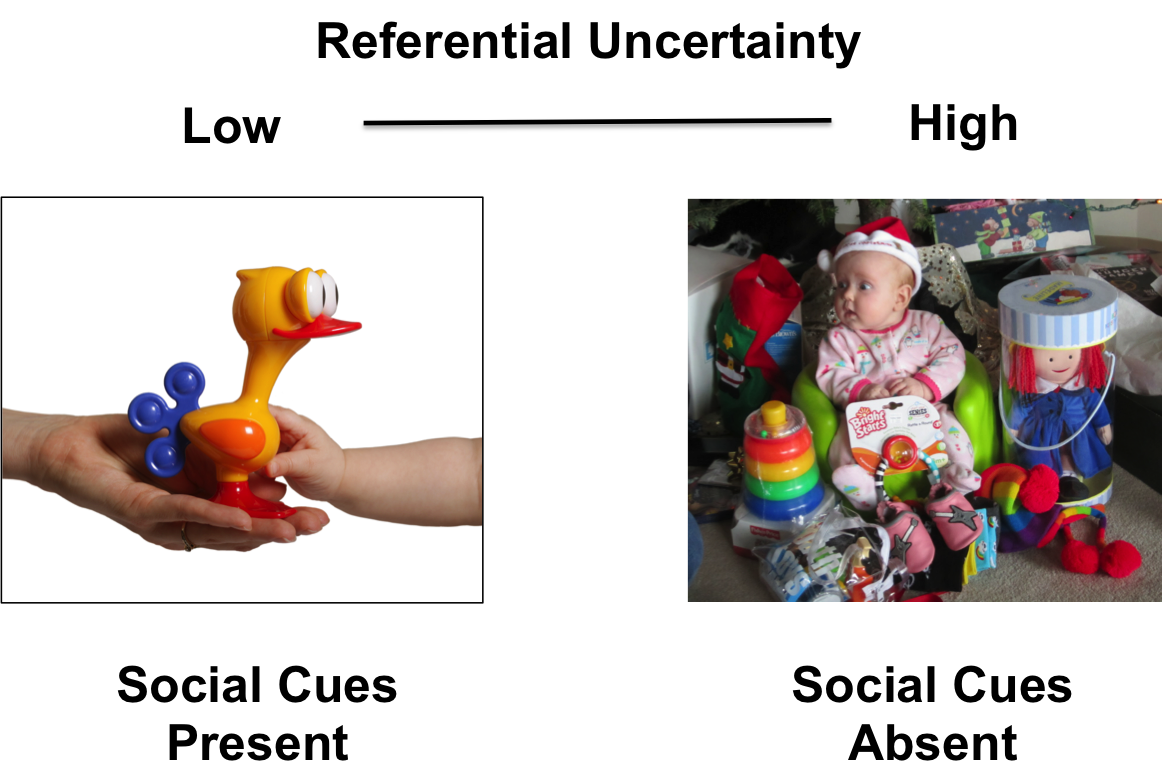
\includegraphics[scale=0.45]{plots_figures/ref_uncertainty.png}}
	\caption{Two real-world word learning contexts located on different ends of a continuum from low to high referential uncertainty. If uncertainty is low, perhaps learners only need to track a single candidate word-object link, but if uncertainty is high, learners might track multiple word-object links in order to identify the correct meaning over time.}
\end{figure}
%
\newpage

Experimental work shows that children as young as 16 months are sophisticated intention-readers, preferring to map novel words to objects that are the target of a speaker's gaze and not their own \cite{baldwin1993infants,baldwin2001links}. More recent research suggests that labeling contexts accompanied with social cues provide children with clear visual access to objects during naming, creating an ideal word-learning situation \cite{yu2012embodied}. Moreover, correlational data show strong links between early intention-reading skills (e.g., gaze following) and later vocabulary growth in typically-developing children \cite{brooks2008infant} and children diagnosed with autism \cite{mundy1990longitudinal}. But, not all of children's labeling experiences occur in rich social contexts. So how might children, in the absence of social cues to reference, learn new words? 

Associative accounts of word-learning argue that word-object co-occurrence statistics allow the learner to reduce referential uncertainty over time  \cite{smith2000learning}. Returning to our example, even if the speaker's referential intent is unclear in-the-moment, the child could track the co-occurrence of the new word with several of the toys in the visual scene. And since over time that word is more likely to co-occur with it's referent, the child could use this information to identify the correct word-object mapping. 

Research with young infants shows that they are capable of learning from statistical information in both the auditory \cite{saffran1996statistical} and visual \cite{fiser2002statistical} domains. And recent experimental work provides evidence that adults and children are able to rapidly learn words by tracking co-occurrence statistics across multiple, ambiguous exposures \cite{smith2008infants, vouloumanos2008fine}. For example, \citeA{smith2008infants} taught children three novel words simply by repeating consistent novel word-object pairings across 10 ambiguous exposure trials.  Importantly, there was no way for children to infer the correct meaning of the novel word on any one trial, but, over time, they could use co-occurrence statistics to identify the correct mappings. Moreover, recent computational models suggest that cross-situational learning can scale up to learn adult-sized lexicons, even under conditions of considerable referential uncertainty \cite{smith2011cross}.

Hence, both social cues and cross-situational statistics can sufficiently reduce referential uncertainty, allowing word learning to proceed. But, there is still considerable debate over a) the exact computation that cross-situational learners perform and b) how learners integrate social and statistical information. Do learners store information about one or several alternative word-object links? Does social information influence these representations? In the next section, we review these debates and suggest that the type of representation that learners store is modulated by the presence of social information during learning. 

%%%%%%%%% SINGLE VS. MULTIPLE  REFERENT TRACKING %%%%%%%%% 

\section{Representations underlying cross-situational word-learning}

Researchers studying cross-situational word-learning generally do not disagree about the computational-level problem that learners must solve. That is, the learner must take in input in the form of co-occurrences between objects and words and perform a statistical computation over that input, with word-learning occurring as a result. However there is disagreement about the cognitive processes that make use of co-occurrence statistics \cite{smith2014unrealized}. 

Some evidence suggests that cross-situational learners track multiple word-object mappings, storing these links in a co-occurrence matrix with different association strengths \cite{vouloumanos2008fine, mcmurray2012word, yurovsky2014role}. Other evidence suggests that cross-situational learning is better characterized as a a single hypothesis tracking mechanism, which stores a single word-object link that is either verified or rejected by subsequent co-occurrence information \cite{trueswell2013propose,medina2011words}. Recent experimental and modeling work directly tested the viability of these two accounts and found that an integrative model best captured participants' learning behavior \cite{yurovsky2014algorithmic}. Moreover, Yurovsky and Frank showed that learners co-occurrence tracking is influenced by the attentional and memory demands present during learning: when demands increased, learners were more likely to shift to single referent tracking. 

While Yurovsky and Frank did not set out to explore the role of social information in cross-situational word-learning, their paradigm is well-suited for asking this question. Previous work with infants shows that social cues can: a) produce better spatial learning of audiovisual events \cite{wu2010no}, b) better recognition of a cued object \cite{cleveland2007joint}, and c) differential encoding of an object's featural or spatial information \cite{yoon2008communication}. This work, taken together with the research reviewed in Section 1, suggests that social cues could play an important role in modulating the input to cross-situational learning mechanisms.

Here we directly test the role of social information by modifying Yurovsky and Frank's paradigm to include a social cue to reference: eye gaze. We explore the effects of eye gaze at different levels of referential uncertainty by parametrically manipulating a) the number of referents present during learning and b) the interval between successive exposures to the same word. At all levels of difficulty, learners were less likely to track multiple word-object links when social cues were present, suggesting a tradeoff between reducing uncertainty during labeling and the type of representations that learners store.  


%%%%%%%%% EXPERIMENT  %%%%%%%%% 


\section{Experiment}

We set out to test the effect of social cues on cross-situational learning at different levels of attention and memory demands. The design closely follows Yurovsky and Frank's paradigm: participants saw a series of ambiguous word-learning trials that consisted of a set of novel objects (either 2, 4, 6, or 8) and heard a novel word. They were asked to make guesses about which object went with each word. In subsequent test trials, participants heard the novel word again after different numbers of intervening trials (0, 1, 3, and 7), this time paired with another set of novel objects. One of the objects in the set was either the participant's initial guess (Same trials) or one of the objects that was \emph{not} the initial guess (Switch trials). While both single and multiple referent trackers could succeed on Same trials, only participants who encoded multiple objects during their first encounter could succeed on Switch trials. This provides a direct test of whether learners track multiple alternatives.

In the current work, we add a speaker who directs her gaze towards one of the objects during the initial exposure trial, potentially reducing referential uncertainty. This allows us to explore the interaction between social information and referent tracking during cross-situational learning. 

\subsection{Participants}

This experiment was posted to Amazon Mechanical Turk as a set of
Human Intelligence Tasks (HITs) to be completed only by participants with US IP
addresses and an approval rate above 95\%. Each HIT paid 30 cents. Approximately 50-75 HITs were posted for each of the 32 conditions (4 referents X 4 intervals X 2 social conditions) for total of approximately 2200 paid HITs. If a participant
completed the experiment more than once, he or she was paid each time but only data
from the first HITs completion was included in the final data set. In
addition, data was excluded from the final sample if participants did not give correct
answers for familiar trials (excluded 5 HITs).

%
\begin{figure} [H]
	\centering
	\fbox{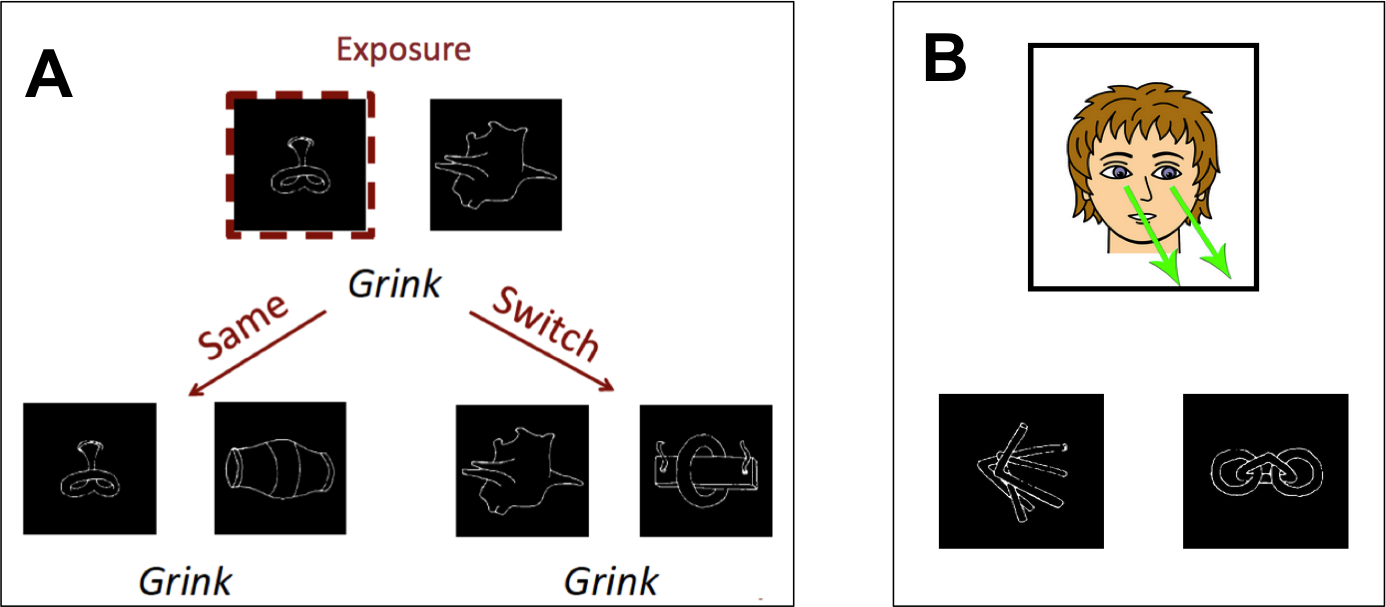
\includegraphics[scale=0.6]{plots_figures/stimuli2.png}}
	\caption{Experimental stimuli. Panel A shows a schematic of the trials that participants saw in the experiment. On Exposure trials, participants saw a set of novel objects and heard a novel word. Participants were asked to guess it's correct referent. After the Exposure trial, participants either saw a Same or a Switch trial. On Same trials, the set of referents contained the participant's previous guess. On Switch trials, the set of referents contained one of the objects that was not the participant's initial guess. Panel B shows an Exposure trial in the Social condition. In the Non-social condition, the speaker looked straight ahead during exposure. During test trials (both Same and Switch) the speaker looked straight ahead.}
\end{figure}
%

\subsection{Stimuli}

Stimuli for the experiment consisted of black and white pictures of familiar
and novel objects, a schematic drawing of a human interlocutor, and audio recordings of familiar and novel words. Pictures of 32 familiar objects spanning a range of categories (e.g. squirrel, truck, tomato, sweater) were drawn from the set constructed by \citeA{snodgrass1980standardized}. Pictures of distinct but
difficult to name objects were drawn from the set of 140 first used in \citeA{kanwisher1997locus}. For ease of viewing on participants' monitors, pixel values for all pictures were inverted so that they appeared as white outlines on black backgrounds (see Figure 2). Familiar words consisted of the labels for the familiar objects as produced by AT&T Natural VoicesTM (voice: Crystal). Novel words were 1-3 syllable pseudowords obeying the rules of English phonotactics produced using the same speech synthesizer.

A schematic drawing of a human speaker was chosen for ease of manipulating the direction of eye gaze, the social cue of interest in this study (see Figure 2). Images were created using Adobe Photoshop. Since this task was performed over the internet and participants' screen sizes might be small, we added large, green arrows to ensure that participants would know the direction of the speaker's eye gaze.


\subsection{Design and Procedure}
Participants were exposed to a series of trials in which they heard a speaker say a novel word, saw a set of novel objects, and were asked to guess which object went with the word. After a written explanation of the task, participants completed
four practice trials. On each practice trial, they heard the speaker say a
familiar word while looking at that object among a set of other familiar objects.
On the first two trials, participants were asked to find the squirrel, and the correct answer
was in the same position on each trial. On the next two trials, participants were asked to
find the tomato, and the correct answer switched positions from the first to the second
trial (in order to ensure that participants understood that the on-screen position was not
an informative cue to the correct target). These trials also served to screen for participants
who did not have their audio enabled or who were not attending to the task.

After these Familiarization trials, participants were informed that they would now hear
novel words, and see novel objects, and that they should continue selecting the correct
referent for each word. Participants each heard eight novel words twice. Participants saw either 2, 4, 6, or 8 referents on each trial, and the two trials for each word occurred back-to-back. Four of these follow-up trials were Same trials in which the referent that participants selected on the exposure trial appeared again amongst the set of objects. The other four were
Switch trials in which one of the referents in the set was selected randomly from the objects
a participant did not select on the previous Exposure trial. All other referents were
completely novel on each trial. 

Critically, on Exposure trials the interlocutor's eye gaze was directed and thus informative, but on Same/Switch trials her eye gaze was uninformative. Participants were randomly assigned to the Social or Non-social conditions. In the Social condition, eye gaze was informative; in the Non-social condition, eye gaze was uninformative throughout the task. To indicate that participants' selections had been registered, a red dashed box appeared
around the object they selected for 1 second after their click was received. This box
appeared around the selected object whether or not it was the "correct" referent.

%%%%%%%%% STUDY - RESULTS  %%%%%%%%% 

\section{Results}

\subsection{Exposure trials}

First, we wanted to ensure that our social cue manipulation was effective. To do this, we compared participant's performance on Exposure trials in the Social condition against the distribution expected if participants were selecting randomly (defined by a Binomial distribution with four trials and a probability of success of $\frac{1}{\# Referents}$). Figure 3, Panel A shows participants' accuracies in selecting the object that was the target of the speaker's gaze. In all four Referent conditions, participants' responses differed from those expected by chance, exact binomial  $p$(two-tailed) $< .001$, suggesting that the social cue effectively directed attention to the target referent.

%
\begin{figure}[H]
	\centering
	\fbox{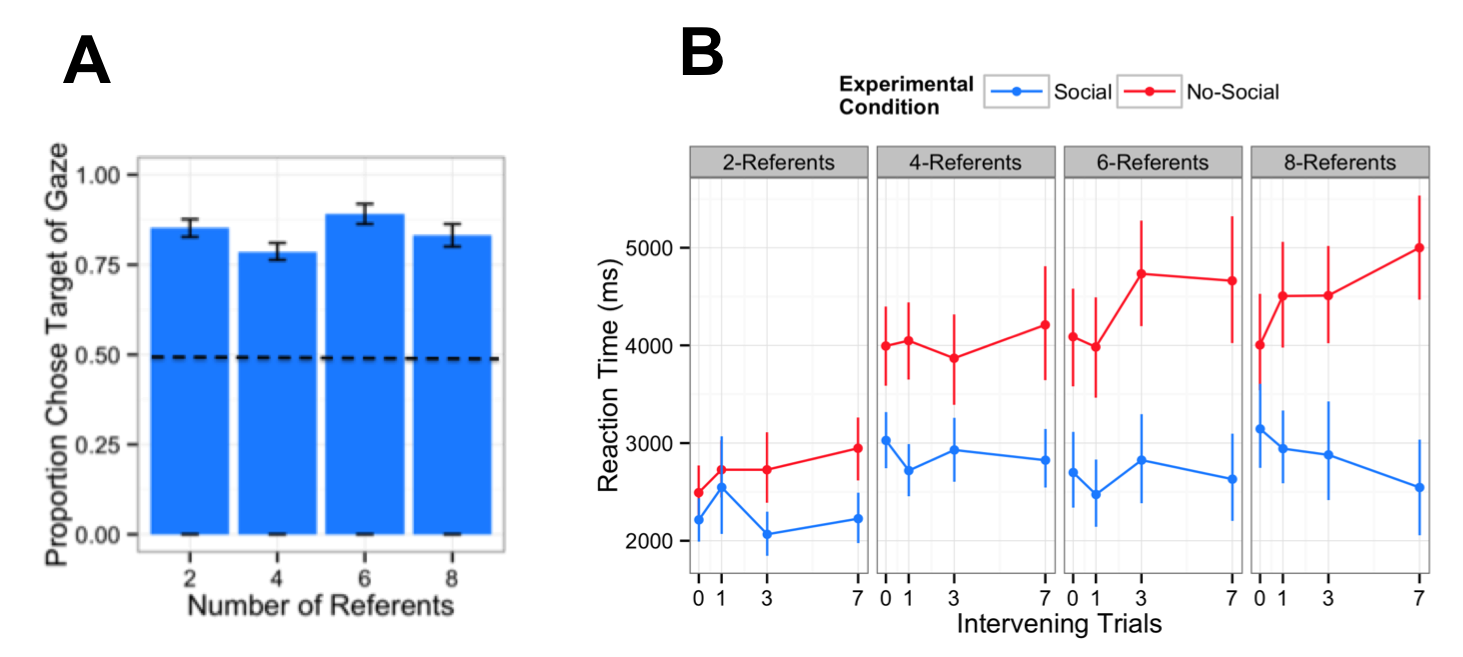
\includegraphics[scale=0.4]{plots_figures/exp_all.png}}
	\caption{Data from exposure trials in the Social condition. Panel A shows participants' accuracy across the four referent conditions. Participants reliably selected the target of the speaker's eye gaze, suggesting that the social cue was effective. Panel B shows participants' reaction times on exposure trials. Participants responded faster in the Social condition.}
\end{figure}
%

Participants' reaction times on exposure trials are shown in Figure 4, Panel B. Because these trials were self-paced participants' response teams are a proxy for processing of the stimuli. To quantify the effect of each factor on reaction time, we fit a linear regression model to the data from the full dataset (Supplementary Table 1 shows model output). There were main effects of Condition and Referents such that participants responded faster in the Social condition and slower as the number referents increased. The two-way interaction between Condition and Interval was significant such that as the number of referents increased, participants in the Non-social conditions responded slower. This analysis provides additional support that our social cue was effective, and suggests that reduced processing time could be a possible mechanism for the effect of social cues on participants' performance at test. 

\subsection{Test trials}
To analyze performance on Test trials, we compared the distribution of correct responses made by each participant to the distribution expected if participants were selecting randomly (defined by a Binomial distribution with four trials and a probability of success of  $\frac{1}{\# Referents}$). Figure 4 shows participants' accuracies in identifying the referent of each word in all conditions for both kinds of trials (Same and Switch) and in each condition (Social and Non-social). We replicate the finding from \citeA{yurovsky2014algorithmic}: at all Referent and Interval levels, both for Same and for Switch trials, participants' responses differed from those expected by chance (smallest $\chi^{2}(4) = 12.07, p < .01$). Thus, learners encode more than a single hypothesis in ambiguous word learning situations, even under high attentional and memory demands and in the presence of a social cue to reference. 

%
\begin{figure}[H]
	\centering
	\fbox{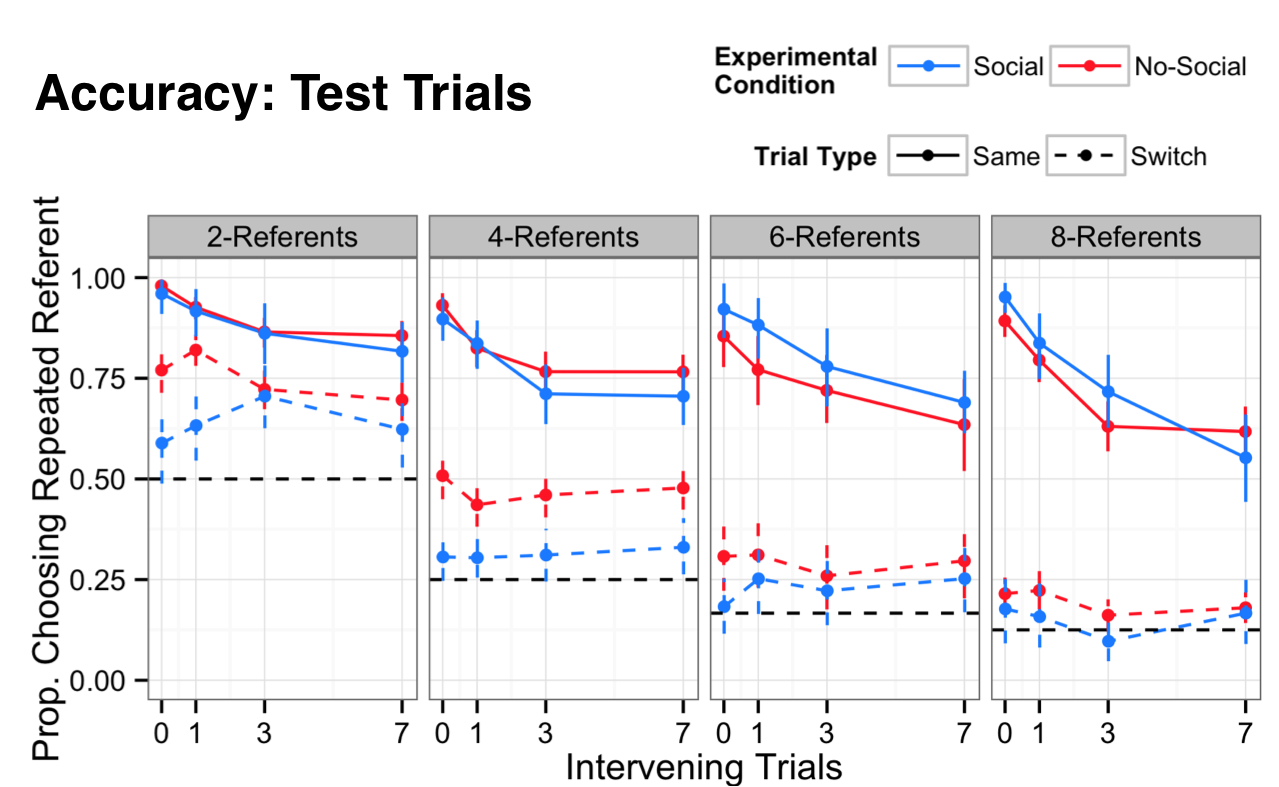
\includegraphics[scale=0.40]{plots_figures/acc_test.png}}
	\caption{Accuracy on test trials for both trial types (Same and Swtich) and experimental conditions (Social and Non-social). Each datapoint represents approximately 50-75 participants. Error bars indicate 95\% confidence intervals computed by non-parametric bootstrap. Learners tracked multiple referents at all levels of memory and attention, but participants performed worse on Switch trials in the Social condition.}
\end{figure}
%

Does participants' learning behavior look different in the presence of social cues? To quantify the effect of each factor on word learning, we fit a mixed-effects logistic regression model to the data from the full dataset \cite{baayen2008mixed}. Table 1 shows the model output. This analysis showed significant main effects of Number of Referents, Interval, Trial Type, and Condition. In addition, the model showed a significant two-way interaction between Referents and Trial Type, Interval and Trial Type, Condition and Referent, and, importantly, Condition and Trial Type. Thus, word learning occurred at almost all levels of referential ambiguity and memory demands, but Switch trials were more challenging in the Social condition across all levels of uncertainty. 

% latex table generated in R 3.1.0 by xtable 1.7-3 package
% Mon Jun  2 04:19:58 2014
\begin{table}[H]
\centering
\caption{\textbf{Mixed-effects logistic regression model output}}
\begin{tabular}{lrrrrl}
 Predictor & Estimate & Std. Error & $z$ value & $p$ value &  \\ 
  \hline
Intercept & 4.18 & 0.20 & 20.42 & 0.00 & *** \\ 
  Switch Trial & -1.58 & 0.17 & -9.25 & 0.00 & *** \\ 
  Social Condition & -0.47 & 0.22 & -2.18 & 0.03 & * \\ 
  Log(Interval) & -0.60 & 0.08 & -7.43 & 0.00 & *** \\ 
  Log(Referents) & -0.69 & 0.08 & -8.44 & 0.00 & *** \\ 
  Switch Trial*Social Condition & -0.57 & 0.10 & -5.60 & 0.00 & *** \\ 
  Switch Trial*Log(Interval) & 0.52 & 0.04 & 11.97 & 0.00 & *** \\ 
  Switch Trial*Log(Referent) & -0.63 & 0.06 & -9.77 & 0.00 & *** \\ 
  Social Condition*Log(Interval) & 0.08 & 0.05 & 1.54 & 0.12 &  \\ 
  Social Condition*Log(Referent) & 0.18 & 0.08 & 2.21 & 0.03 & * \\ 
  Log(Interval)*Log(Referent & 0.00 & 0.03 & 0.03 & 0.98 &  \\ 
   \hline
\end{tabular}
\raggedright

The model was specified as: $Correct \sim (trialType + condition + Log(Interval) + Log(Referents))^2 + (trialType | subject)$
\end{table}

We also analyzed reaction times on test trials. There were main effects of Trial Type and Referents: participants responded faster on Switch trials and slower as the number of referents increased. Several two-way interactions were significant: Trial Type by Condition, Trial Type by Interval, Trial Type by Referent, and Interval by Referent. Focusing on the Trial type by Condition interaction, participants were slower to respond in the Social condition and this effect increased as the number of referents increased.    

%
\begin{figure}[H]
	\centering
	\fbox{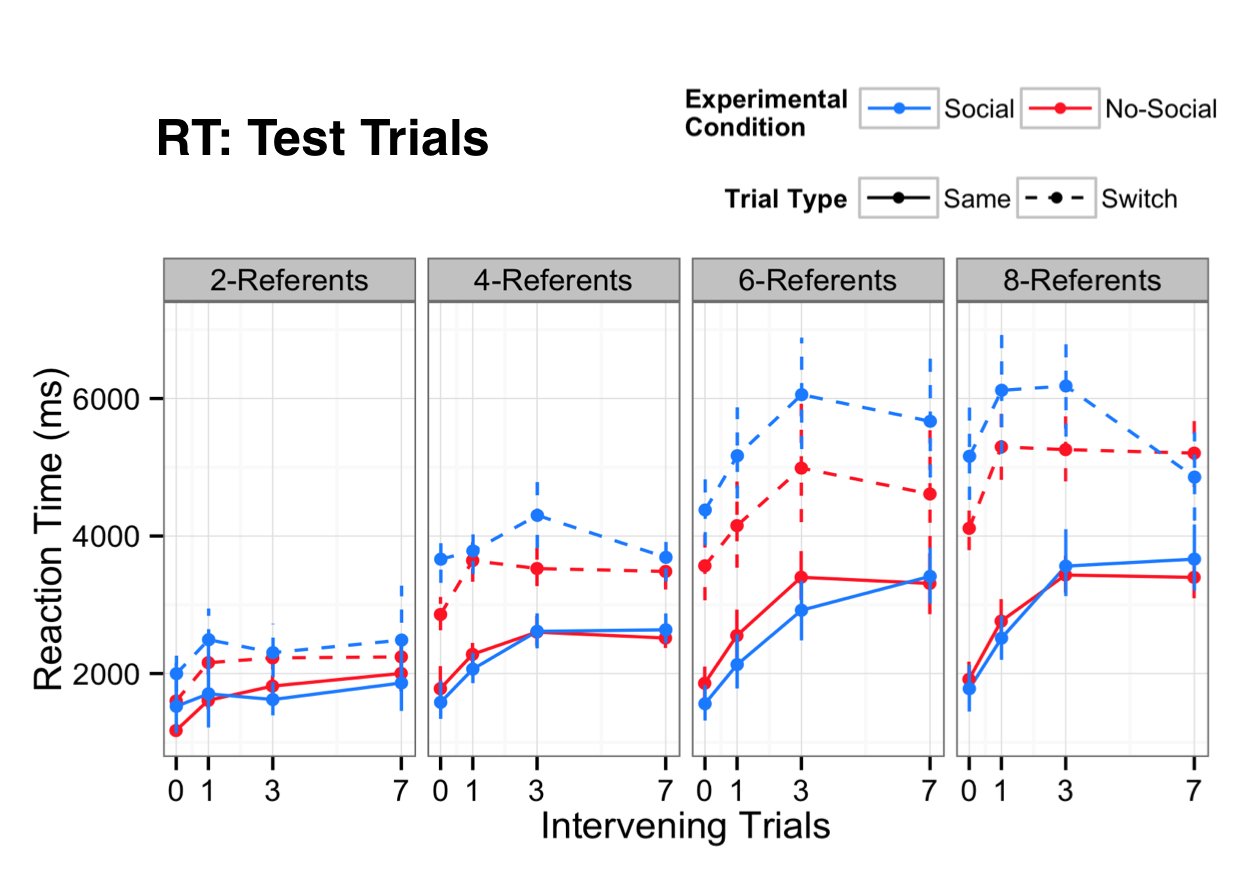
\includegraphics[scale=0.45]{plots_figures/rt_test.png}}
	\caption{Reaction time on test trials for both trial types (Same and Switch) and experimental conditions (Social and Non-social). Participants were slowest to respond on Switch trials in the Social condition, suggesting that these were the most challenging trials for participants. This provides additional evidence that the social cue reduced participants tracking of alternative word-object links.}
\end{figure}
%


Taken together, the Accuracy and Reaction time analyses provide strong evidence that the presence of a social cue modulated participants' learning behavior, making participants less likely to track multiple word-object links. In the next section, we formalize this idea with a computational model of participants' behavior on this task.

%%%%%%%%% MODEL  %%%%%%%%% 

\section{Model}

To formalize the influence of social cues on cross-situational word-learning, we build upon a computational model originally proposed by \citeA{frank2009using} and extended by \citeA{yurovsky2014algorithmic}. First, we review these two models. Then we present a series of simulations that allow us to generate model predictions across different parameters with the goal of capturing participants' learning behavior on our task.

\citeauthor{frank2009using} define the word-learning problem by a set of variables and probabilistic dependencies that link these variables. The learner observes a set of situations \emph{S} in the world, which consist of two observed variables: objects (\emph{O}) and words (\emph{W}), and one unobserved variable: the speaker's referential intention (\emph{I}). The learner's task is to infer the lexicon (\emph{L}) that is most likely to have generated the set of observed situations. Formally, this learning task can be defined as a problem of Bayesian inference: 
%
\begin{equation}
\label{1}
P(L|S) \propto P(S|L)P(L)
\end{equation}
%
The likelihood term ($P(S|L)$) captures the learner's assumptions about the task. Each situation (\emph{S}) includes a word, a set of objects, and the speaker's referential intention (\emph{I}). Thus, $P(S|L)$ can be expanded and the probability of the lexicon can be given as: 
%
\begin{equation}
\label{2}
P(L|S) \propto \prod\limits_{s \in S}  P(W_s, I_s, O_s|L)P(L)
\end{equation}
%
Because referential intention mediates the relationship between words and objects, the likelihood term can be rewritten as:
%
\begin{equation}
\label{3}
P(L|S) \propto \prod\limits_{s \in S}  P(W_s|I_s, L)P(I_s|O_s)P(L)
\end{equation}
%
The prior probability of a lexicon is defined as: $P(L_o) \propto \frac{1}{|L_o|}$, which is a parsimony prior that favors lexicons with fewer words referring to the same object. 

 \citeA{yurovsky2014algorithmic} then extended this computational level description to include cognitive constraints, allowing them to provide an algorithmic-level account of their data. In this model, memory was defined by a power function that took into account the interval between successive exposures to a word and the strength of initial encoding. The $\gamma$ parameter scaled to the encoding strength and the $\lambda$ parameter defined the rate of decay.
%
\begin{equation}
\label{4}
M(L_o) =  \gamma L_ot^{-\lambda}
\end{equation}
%

Attention was defined in terms of the learner's belief about $P(I|O)$: the probability of the speaker's intent to refer to each object in the set. The $\sigma$ parameter captures the amount of probability mass that the learner places on each referent during the initial exposure to a new word. The strength of the learner's belief about $P(I|O)$ in turn directly influences the strength of initial encoding ($\gamma$). 

Finally, \citeA{yurovsky2014algorithmic} provided a choice rule to describe how learners select among the objects on each test trial: learners choose the correct referent with probability proportional to their memory for its lexical entry, and otherwise choose randomly among the set of referents.\footnote{This formulation is equivalent to using Luce's Choice Axiom \cite{luce1959individual} in which the target has strength  $M(L_{o}) + \frac{1-M(L_{o})}{|O|}$ and each foil has strength $\frac{1-M(L_{o})}{|O|}$.} 

\begin{align}
P(Correct) = M(L_{o}) + \frac{1-M(L_{o})}{|O|}
\end{align}

Using these three parameters -- encoding strength, decay, and attention -- we can model different types of learning.  At $\sigma = 1$, the learner is placing all of their attention on one word-object mapping (i.e. a single hypothesis tracking strategy). At $\sigma = \frac{1}{|O|}$, the learner is distributing the probability mass across all possible word-object mappings equally (i.e. a parallel statistical accumulator strategy). Figure 6 shows the model predictions for these two learning strategies\footnote{For clarity, here we just model the 4-referent condition.}. 

%
\begin{figure}[H]
	\centering
	\fbox{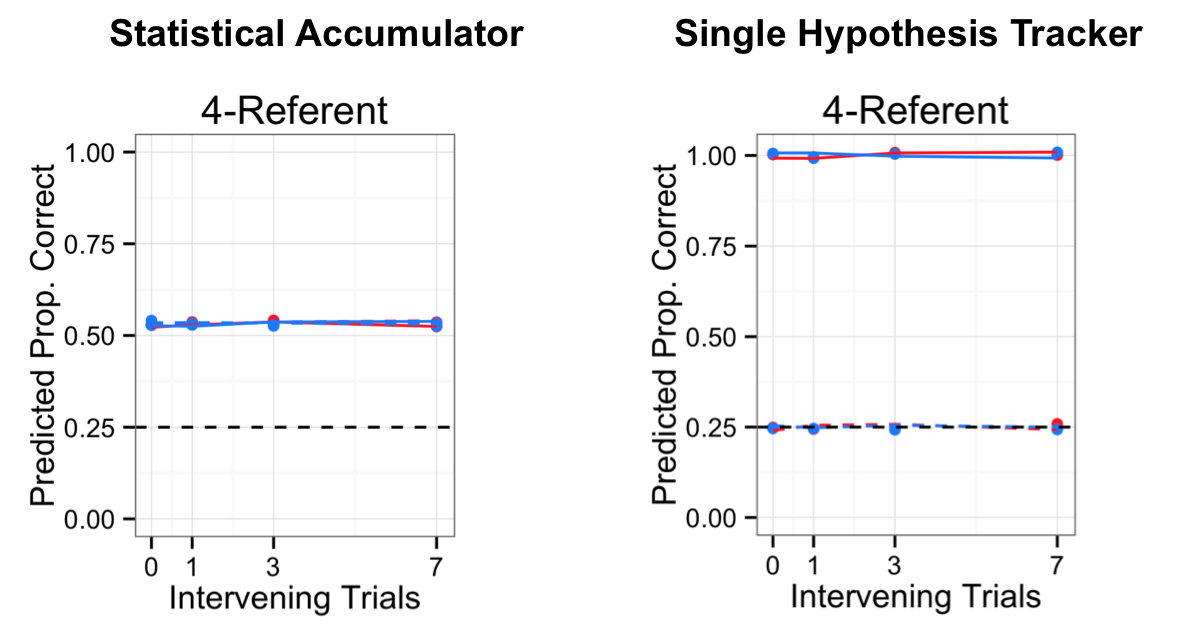
\includegraphics[scale=0.55]{plots_figures/model_sims1.png}}
	\caption{Model predictions for the single hypothesis tracking account ($\sigma=1$) and the pure statistical accumulator ($\sigma=\frac{1}{|O|}$). These two models represent the ends of a continuum of potential learning strategies.}
\end{figure}
%

The Parallel Accumulator model predicts indistinguishable performance on Same and Switch trials because the learner is allocating belief evenly across referents. In contrast, the Single Hypothesis Tracking model predicts perfect performance on Same trials and chance performance on Switch trials because all belief is concentrated on a single referent. \citeA{yurovsky2014algorithmic} fit the parameters of this model to participants' data and found that an integrated model, allocating a certain amount of attention to a single candidate hypothesis and distributing the rest over the remaining referents best captured learning behavior.  

Using these best fit parameters, we can model the effect of social information as a boost to the $\sigma$ parameter, increasing the amount of belief participants allocate to their initial selection. Figure 7 shows model predictions from this simulation. This model predicts improved performance on Same trials and decreased performance on Switch trials when social cues are present. 


%
\begin{figure}[H]
	\centering
	\fbox{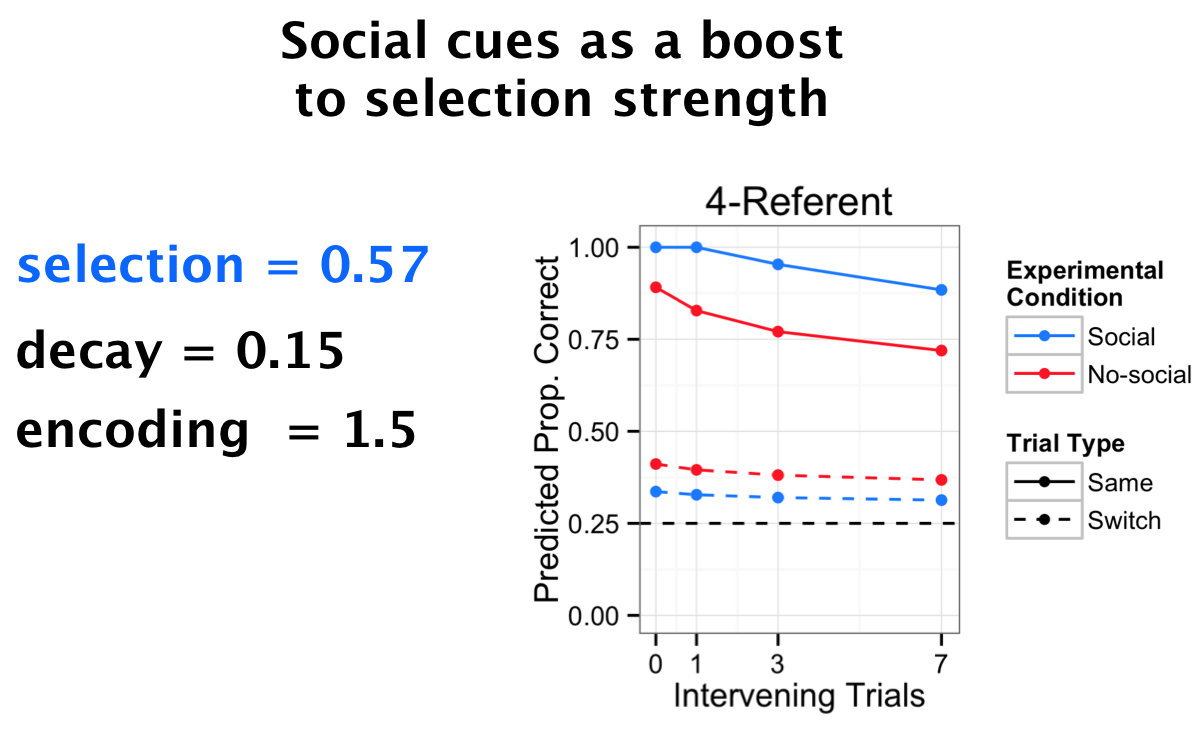
\includegraphics[scale=0.5]{plots_figures/soc_boost.png}}
	\caption{Model predictions from an integrated model with social cues. Parameter values are best fit values from Yurovsky and Frank's experimental data. Social information is modeled as a boost to the selection strength parameter ($\sigma$). This model predicts better performance on Same trials and worse performance on Switch trials in the Social condition.}
\end{figure}
%


To show how this integrated model captures participants' behavior on our task, we plot the model-data fit (Figure 8). Modeling eye-gaze as a "social boost" to attention does capture the main patterns of data -- a cost to performance on Switch trials in the Social condition, and a boost to Same trials. But there is some complexity in the human data (e.g., the interaction between social information and the number of referents) that we are not capturing. Future versions of the model could treat social information as influencing multiple parameters during the learning process, such as attention and strength of initial encoding.  

%
\begin{figure}[H]
	\centering
	\fbox{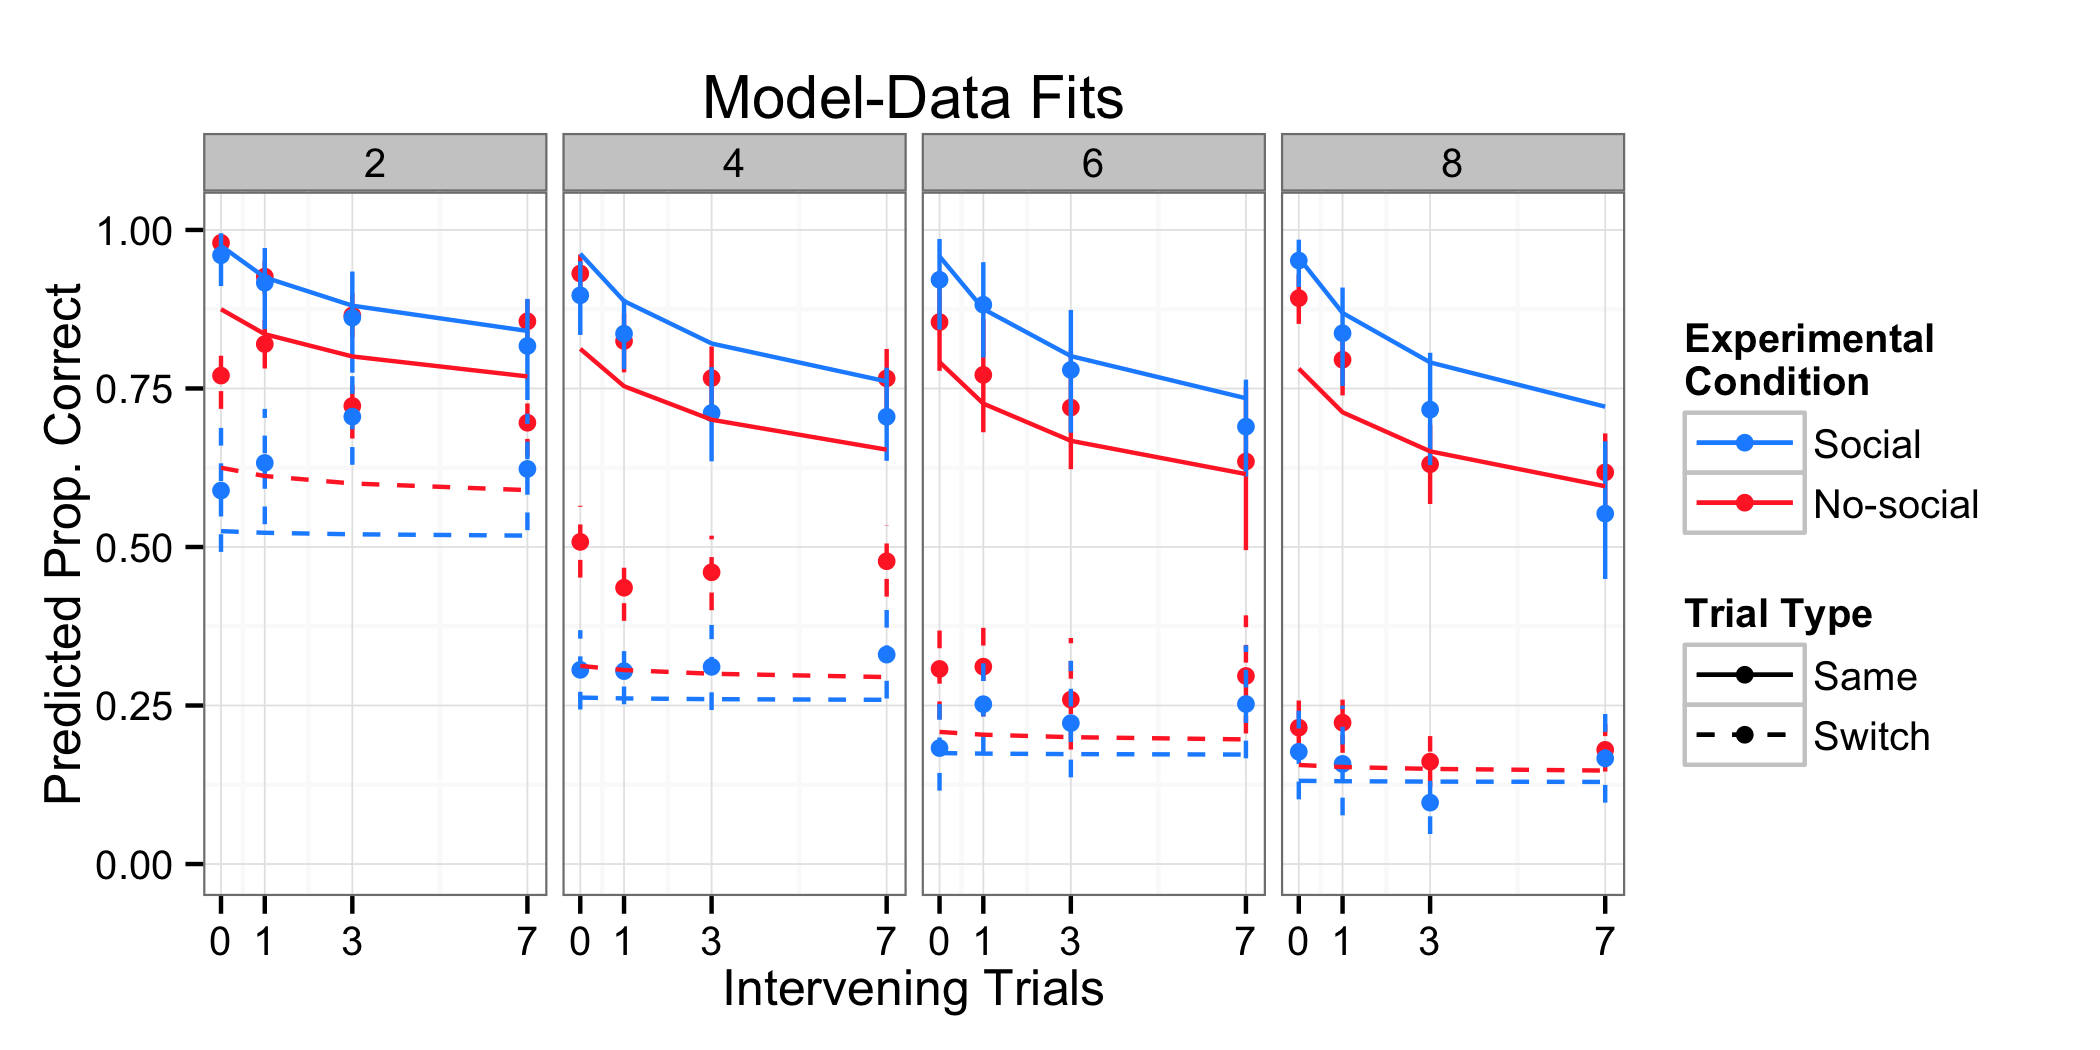
\includegraphics[scale=0.17]{plots_figures/mod_data_fit.png}}
	\caption{Model-data fits. Points are participant data. Each datapoint represents approximately 50-75 participants. Error bars indicate 95\% confidence intervals computed by non-parametric bootstrap. Lines are model predictions from the Integrated Social model.}
\end{figure}
%

Taken together, the experimental data and model predictions provide evidence that the representations that learners store (single vs. multiple referents) during cross-situational word-learning is influenced by their uncertainty during exposure, which in turn can be modulated by the presence of social cues to reference. 

%%%%%%%%% DISCUSSION  %%%%%%%%% 

\section{Discussion}

Social cues and cross-situational statistics provide valuable information about the meanings of new words. Namely, both sources of information can reduce the logically unconstrained number of possible word-object links. But how do social cues, which function in the labeling moment, interact with cross-situational learning, which functions across multiple labeling events? 

Our results suggest that the presence of social information reduces referential uncertainty during learning, which in turn modulates the representations that learners store. When we included eye gaze during exposure trials, learners were less likely to show evidence of tracking multiple word-object links. We attempted to formalize this tradeoff by extending an ideal learning model with cognitive constraints. We modeled social information as a "boost" to the amount of attention allocated to the initial hypothesis during exposure. This captured the tradeoff between reducing referential uncertainty with social cues and reduced tracking of multiple alternatives (i.e., participants worse performance on Switch trials in the Social condition).

How should we characterize the function of social cues during word learning? Recent computational models have attempted to formalize the interaction between social and statistical cues, but talk about social information in fundamentally different ways. For example, in \citeA{yu2007unified}'s Unified Model, social information, is characterized as a ?spotlight? that directs the learner's attention to specific objects, increasing the associative weight given to that word-object pairing.  In contrast, \citeA{frank2009using}'s Intentional model characterizes social information as providing evidence about a speaker?s referential intent, which in turn facilitates word-learning.

Another interesting possibility based on our results is that social information during word learning is a pedagogical cue. Recent experimental work has explored the role of pedagogical information in modulating children's inferences during causal learning tasks. For example, \citeA{bonawitz2011double} have shown that if you present children with a novel toy, which has several different functions (e.g, noise-making), and teach one of those functions, then children are less likely to discover the other functions. Presumably because the learner assumes that if there were other functions to discover, then the teacher would have demonstrated them.  Recent research has formalized pedagogical learning as an inference based on the assumption that a teacher will choose the data most likely to increase the learner's belief in the correct hypothesis \cite{shafto2012learning}. 

The results from our experiment fit well within this framework. In our task, eye gaze provided additional information about the inference the learner should make (i.e., the correct word-object mapping), and as a result learners were less likely to show evidence of tracking alternatives. It is interesting to consider if young learners make pedagogical inferences to facilitate word-learning. Experimental work with 4-year-olds shows that children will generalize the meaning of novel words differently depending on if the objects are sampled by a knowledgeable teacher or by the learner themselves \cite{xu2007sampling}. More recent research has shown that that even infants are sensitive to the sampling process \cite{} and use pedagogical cues to make different assumptions about the generalizability of incoming information \cite{csibra2009natural}. A promising area for future research is to explore whether pedagogical cues modulate early cross-situational learning. Do infants, at the first stages of learning, understand that word-object links are chosen  \emph{for them}, by a \emph{knowledgable} teacher, and are therefore likely \emph{generalizable}?

\section{Supplementary Text}

% latex table generated in R 3.1.0 by xtable 1.7-3 package
% Mon Jun  2 16:17:00 2014
\begin{table}[H]
\centering
\caption{\textbf{Linear regression model output: RT on Exposure Trials}}
\begin{tabular}{lrrrrl}
 Predictor & Estimate & Std. Error & $t$ value & $p$ value &  \\ 
  \hline
Intercept & 1929.77 & 270.29 & 7.14 & 0.00 & *** \\ 
  Social Condition & 174.81 & 381.25 & 0.46 & 0.65 &  \\ 
  Log(Interval) & 3.67 & 142.65 & 0.03 & 0.98 &  \\ 
  Log(Referents) & 791.38 & 121.33 & 6.52 & 0.00 & *** \\ 
  Social Condition*Log(Interval) & 22.52 & 201.99 & 0.11 & 0.91 &  \\ 
  Social Condition*Log(Referent) & -464.94 & 171.83 & -2.71 & 0.01 & ** \\ 
  Log(Interval)*Log(Referent & 84.19 & 64.36 & 1.31 & 0.19 &  \\ 
  Social Condition*Log(Interval)*Log(Referents) & -122.81 & 91.76 & -1.34 & 0.18 &  \\ 
   \hline
\end{tabular}
\raggedright
The model was specified as: 
$RT \sim  Condition + Log(Interval) + Log(Referents)$

\end{table}


% latex table generated in R 3.1.0 by xtable 1.7-3 package
% Mon Jun  2 16:35:28 2014
\begin{table}[H]
\centering
\caption{\textbf{Linear mixed effects model output: RT on Test Trials}}
\begin{tabular}{lrrl}
 Predictor & Estimate & Std. Error & $t$ value \\ 
  \hline
Intercept & 967.45 & 140.43 & 6.89 \\ 
  Switch Trial & -406.79 & 122.41 & -3.32 \\ 
  Social Condition & -129.10 & 186.01 & -0.69 \\ 
  Log(Interval) & 74.68 & 69.61 & 1.07 \\ 
  Log(Referents) & 381.13 & 63.04 & 6.05 \\ 
  Switch Trial*Social Condition & 594.22 & 78.81 & 7.54 \\ 
  Switch Trial*Log(Interval) & -174.55 & 33.69 & -5.18 \\ 
  Switch Trial*Log(Referent) & 923.52 & 49.57 & 18.63 \\ 
  Social Condition*Log(Interval) & 3.87 & 49.60 & 0.08 \\ 
  Social Condition*Log(Referent) & 33.31 & 76.91 & 0.43 \\ 
  Log(Interval)*Log(Referent & 148.42 & 30.92 & 4.80 \\ 
   \hline
\end{tabular}
\raggedright

The model was specified as: 
$RT \sim (trialType + Condition + Log(Interval) + Log(Referents))^2 + (trialType | subject)$

\end{table}


\bibliographystyle{plain}
\bibliography{fyp_p}

\end{document}
